\section{Collections}{\label{Collections}}
In Collections können nur Referenzdatentypen abgelegt werden. Beim Hinzufügen des Elements wird das Objekt selber \textbf{nicht} kopiert,
es wird nur eine Referenz abgelegt. Grundlegende Collections:
\begin{tabular}{l l}
    $\cdot$ \textbf{List} & Folge von Elementen \\
    $\cdot$ \textbf{Set}  & Menge von Elementen \\
    $\cdot$ \textbf{Map}  & Abbildung Schlüssel $\rightarrow$ Werte \\
\end{tabular}

\subsection{Asymptotisches Laufzeitverhalten}
\begin{tabularx}{\linewidth}{l l X} \hline
    \textbf{Laufzeit} & \textbf{Beschr.} & \textbf{Beispiele} \\ \hline
    O(1)        & Konstant      & Indexzugriff Array \\
    O(log(n))   & Logarithmisch & Binärsuche \\
    O(n)        & Linear        & Lineare Suche \\
    O(n*log(n)) & LogLinear     & Schnelle Sortierverfahren: QuickSort, MergeSort \\
    O(n$^2$)    & Quadr.        & Einfache Sortierverfahren: SelectionSort, InsertionSort \\
    O(n$^3$)    & Kubisch       & Matrizen-Multiplikation \\
\end{tabularx}

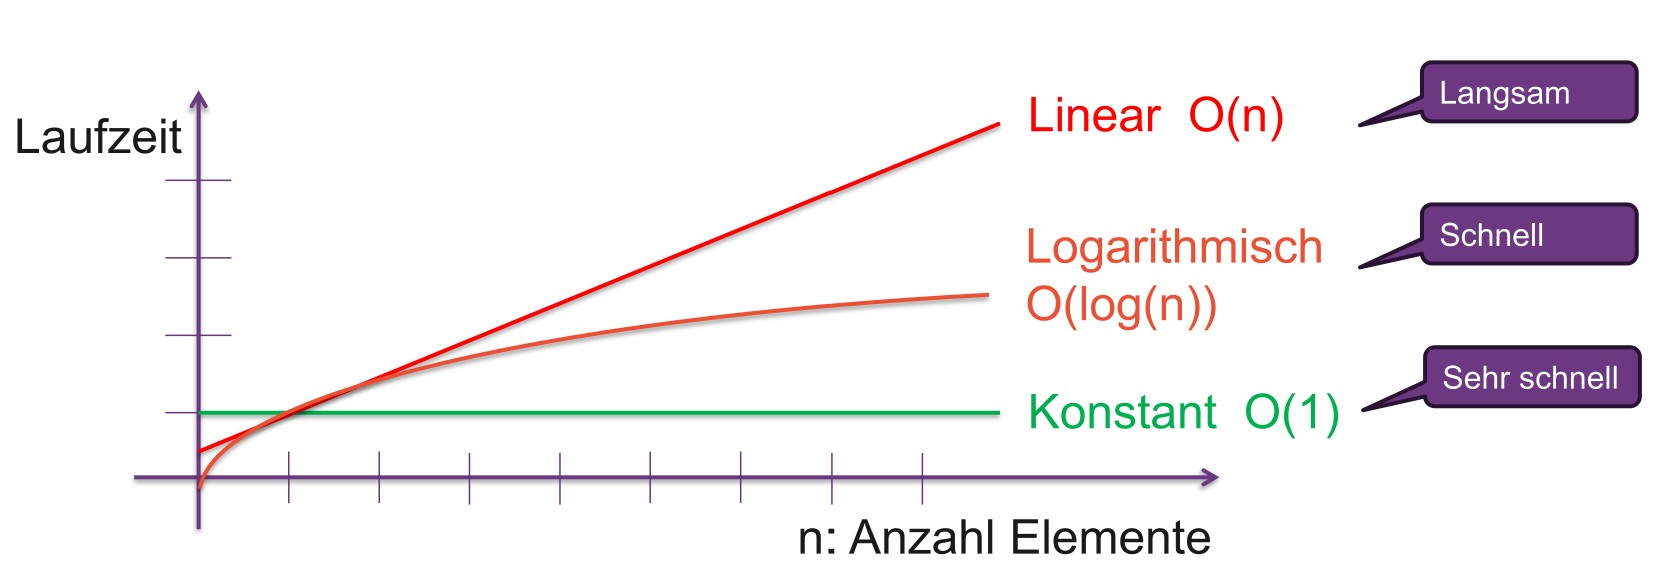
\includegraphics[width=\columnwidth]{pictures/laufzeit-collections.jpg}

\subsection{Wrapper-Objekt}
Um primitive Datentypen in Collections verwenden zu können, müssen sie verpackt (\textit{Wrapping}) werden. Dies geschieht
meist \textbf{implizit}, es muss nur beim Datentyp der Collection definiert werden.
\begin{center}
    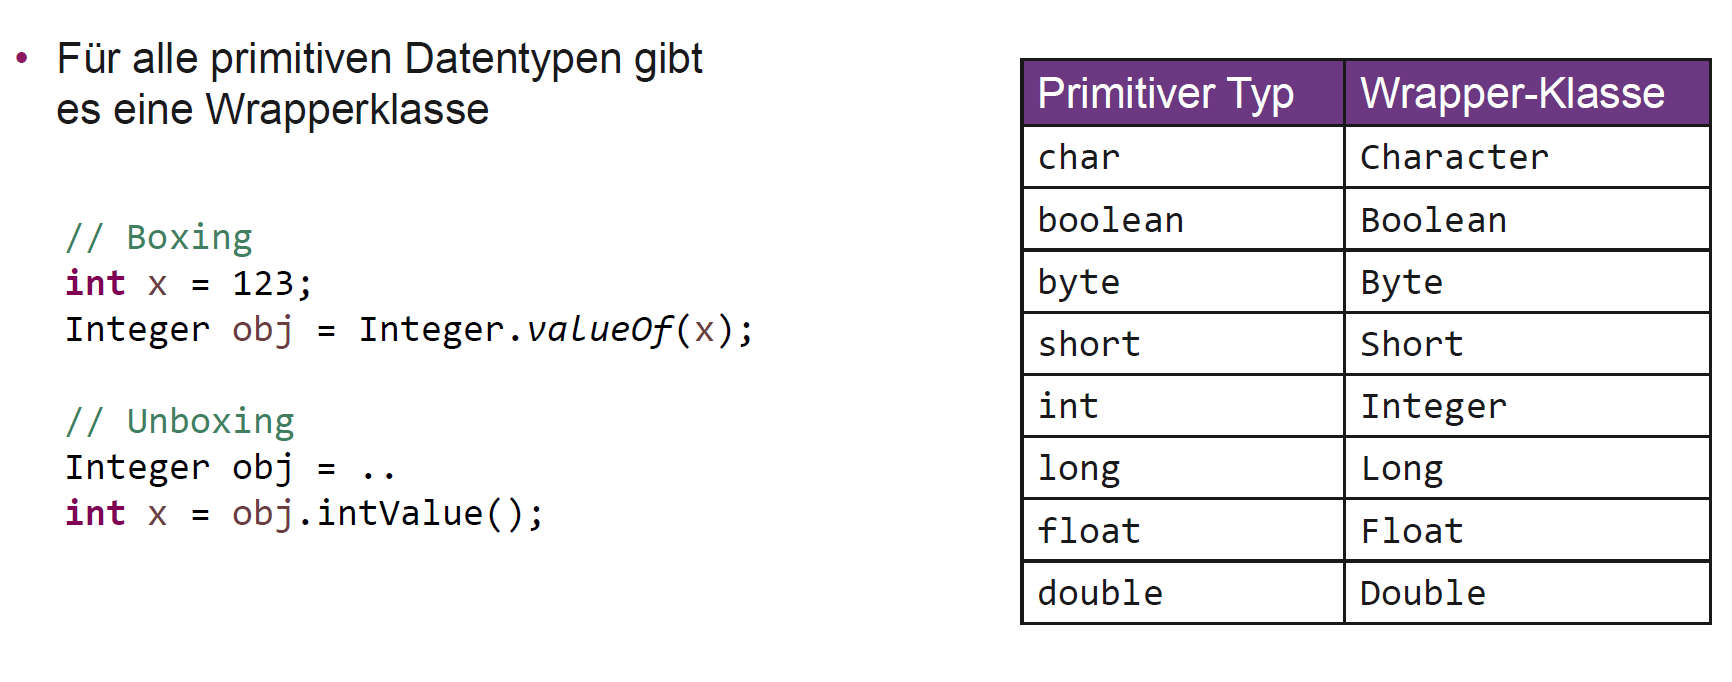
\includegraphics[width=\columnwidth]{pictures/wrapper-klassen.png}
\end{center}

\subsection{ArrayList}
ArrayLists sind eine geordnete Folge von Elementen mit demselben Referenzdatentyp. Elemente können einfach 
hinzugefügt oder entfernt werden. Duplikate oder \verb|null|-Einträge sind möglich\\
Der Zugriff auf Elemente erfolgt über Index (0 ... size()-1). Die Liste verwendet intern ein Array zur Verwaltung der Elemente.
Zu Beginn enthält sie, sofern nicht anders definiert, 10 Elemente und wird bei Erreichen der Kapazität mit Faktor 1.5 mulitpliziert.

\begin{center}
    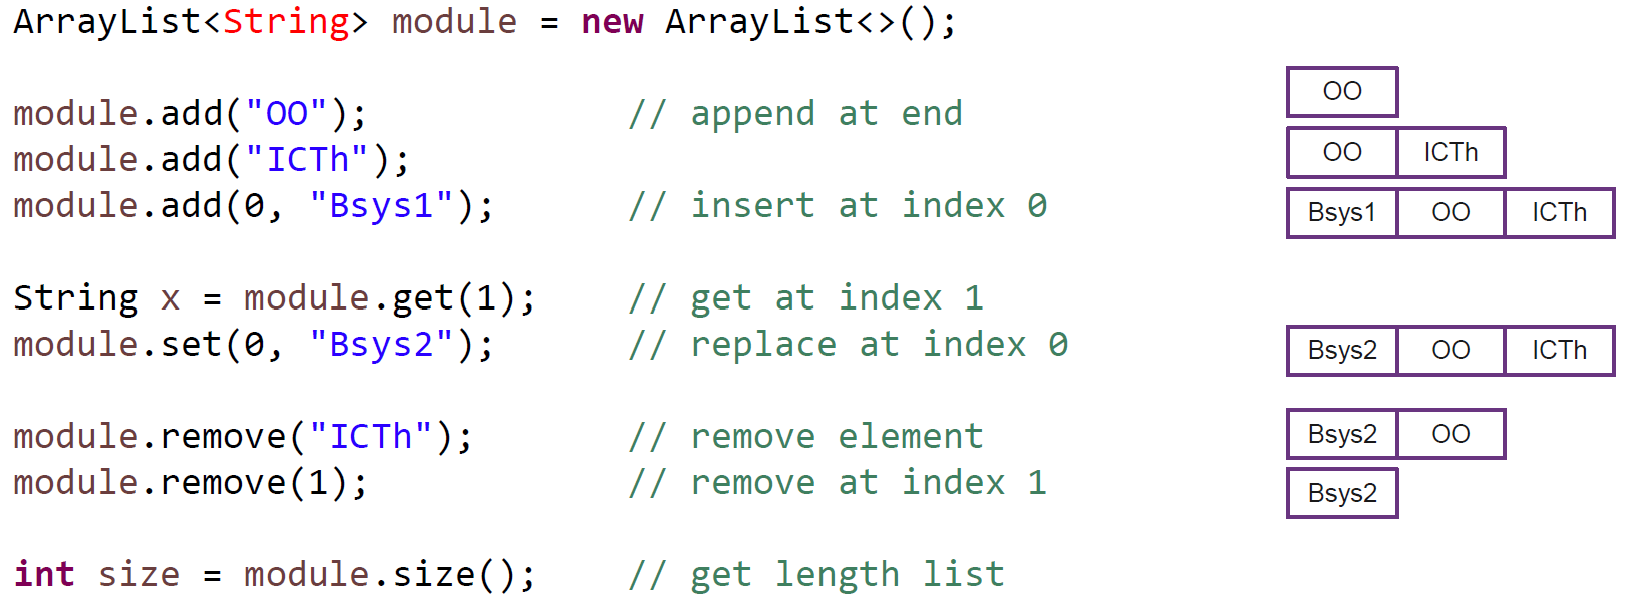
\includegraphics[width=0.9\columnwidth]{pictures/arrayList-bsp.png}
\end{center}

\begin{center}
    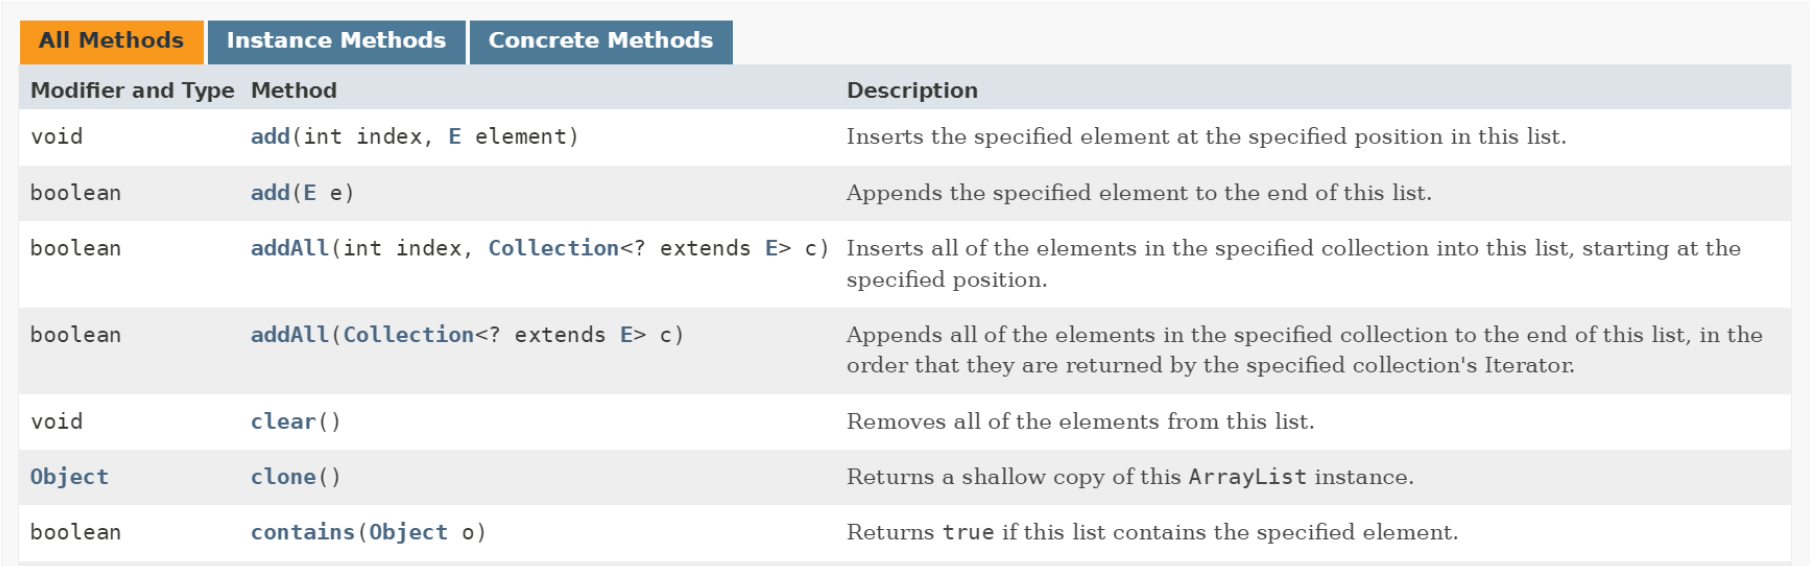
\includegraphics[width=0.9\columnwidth]{pictures/arrayList-api.png}
\end{center}

\subsubsection{ArrayList: Kosten}
\begin{tabular}{l l l} \hline
    \textbf{Operation} & \textbf{Methode} & \textbf{Effizienz} \\ \hline
    Index-Zugriff & get(), set() & \color{green!80!black}Sehr schnell (direkter Zugriff) \\
    Hinzufügen    & add()        & \color{red}Langsam (umkopieren) \\
                  &              & \color{green!80!black}Sehr schnell (ohne umkop.) \\
    Entfernen     & remove(int)  & \color{red}Langsam (umkopieren) \\
    Finden        & contains()   & \color{red}Langsam (durchsuchen) \\
\end{tabular}

\subsection{LinkedList}
Funktioniert ähnlich wie ArrayList. Die Implementierungerfolgt mit einer doppelt-verketteten (vor- und rückwärts) Liste.
Es erfolgt kein Umkopieren beim Einfügen und Löschen von Elementen.

\subsubsection{LinkedList: Kosten}
\begin{tabular}{l l l} \hline
    \textbf{Operation} & \textbf{Methode} & \textbf{Effizienz} \\ \hline
    Index-Zugriff & get(), set() & \color{red} Langsam (traversieren) \\
    Hinzufügen    & add()        & \color{green!80!black}Sehr schnell (Knoten einhängen)\\
    Entfernen     & remove(int)  & \color{red}Langsam in Mitte \\
                  &              & \color{green!80!black}Sehr schnell am Anfang und Ende \\
    Finden        & contains()   & \color{red}Langsam (traversieren) \\
\end{tabular}

\subsection{HashSet vs. TreeSet}
Sets sind Container für Mengen, wobei Duplikate \textbf{nicht} erlaubt sind. Die Gleichheit wird mit \verb|equals()| geprüft.\\
HashSets sind \textbf{unsortiert} und \textbf{oft sehr effizient}\\
\verb|Set<String> firstSet = new HashSet<>();|

\begin{minipage}{0.5\columnwidth}
    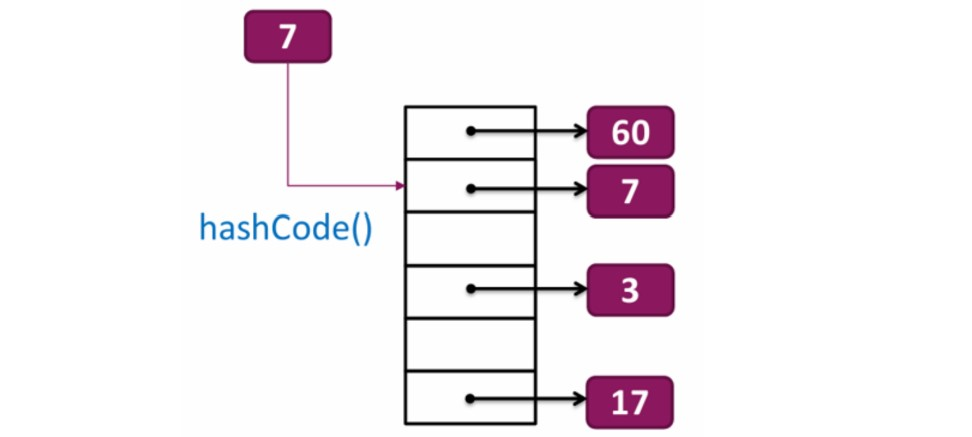
\includegraphics[width=0.9\linewidth]{pictures/hashset.jpg}
\end{minipage}
\hfill
\begin{minipage}{0.45\columnwidth}
    Elemente liefern \verb|hashCode()| konsistent zu \verb|equals()|
\end{minipage}

TreeSets sind \textbf{sortiert} und \textbf{immer effizient}\\
\verb|Set<String> firstSet = new TreeSet<>();|

\begin{minipage}{0.5\columnwidth}
    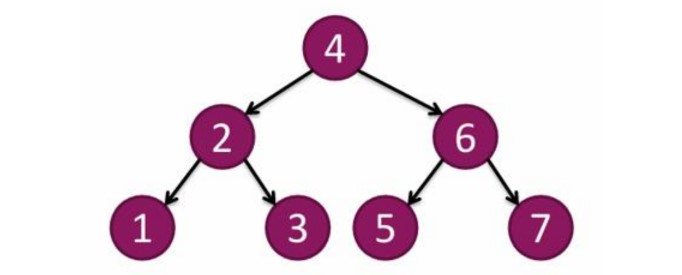
\includegraphics[width=0.9\linewidth]{pictures/treeset.jpg}
\end{minipage}
\hfill
\begin{minipage}{0.45\columnwidth}
    Elemente implementieren \verb|Comparable| und \verb|equals()|
\end{minipage}

\subsubsection{HashSet vs. TreeSet: Kosten}
\begin{tabular}{l l l} \hline
    \textbf{Operation} & \textbf{TreeSet} & \textbf{HashSet }\\ \hline
    Finden      & \color{yellow!75!red} Schnell    & \color{green!80!black}Sehr schnell \\
    Einfügen    & \color{yellow!75!red} Schnell    & \color{green!80!black}Sehr schnell \\
    Löschen     & \color{yellow!75!red} Schnell    & \color{green!80!black}Sehr schnell (nur bei ``guter'' Impl.) \\
    Sortierung  & \color{green!80!black} Ja & \color{red}Nein                    \\
\end{tabular}

\subsection{HashMap vs. TreeMap}
Maps sind für Mengen von Schlüssel-Wert-Paaren. Jedem Schlüssel ist genau ein Wert zugeordnet. Es sind \textbf{keine} doppelten Schlüssel erlaubt. \\
Beispiel:\\
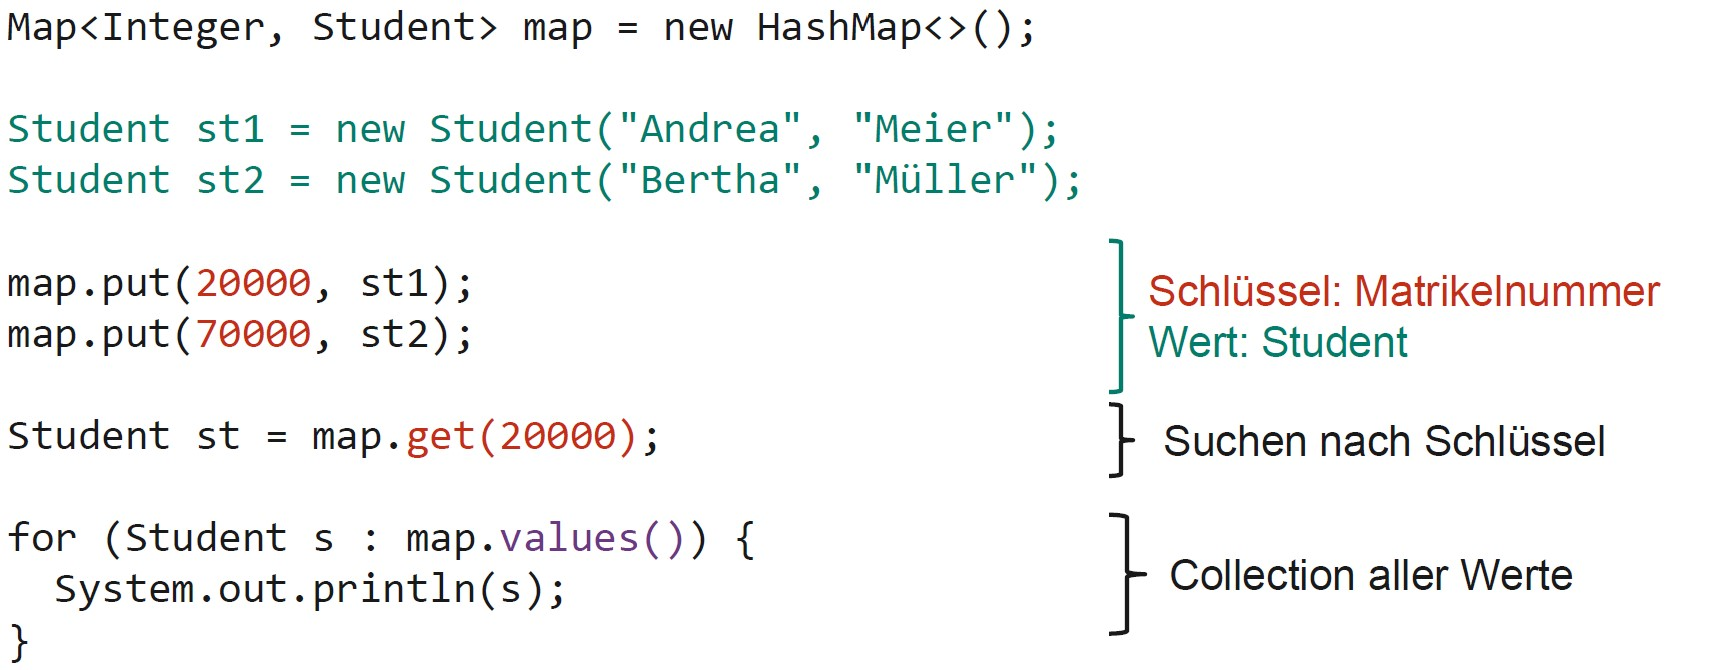
\includegraphics[width=0.7\linewidth]{pictures/map-beispiel.jpg}

HashMaps sind \textbf{unsortiert} und \textbf{oft sehr effizient}\\
\verb|Map<Integer, Student> masters = new HashMap<>();|
\\
\\
TreeMaps sind \textbf{nach Schlüssel sortiert} und \textbf{immer effizient}\\
\verb|Map<Integer, Student> masters = new TreeMap<>();|

\subsubsection{HashMap vs. TreeMap: Kosten}
\begin{tabular}{l l l} \hline
    \textbf{Operation} & \textbf{TreeMap} & \textbf{HashMap }\\ \hline
    Finden      & \color{yellow!75!red} Schnell             & \color{green!80!black}Sehr schnell \\
    Einfügen    & \color{yellow!75!red} Schnell             & \color{green!80!black}Sehr schnell \\
    Löschen     & \color{yellow!75!red} Schnell             & \color{green!80!black}Sehr schnell \\
                &                                           & \color{green!80!black}(nur bei ``guter'' Impl.) \\
    Sortierung  & \color{green!80!black} Ja, nach Schlüssel & \color{red}Nein                    \\
\end{tabular}

\subsection{equals(), Hashing}
Der Operator \verb|==| liefert einen Referenzvergleich, die Methode \textbf{equals()} ist für den inhaltlichen Vergleich.\\
Alle Klassen erben equals() von \textit{Object}. Die Default-Implementation liefert \verb|a == b| (Referenzvergleich). \\
Bei einigen Klassen, z.B. \textit{String, Integer, ...} ist equals() bereits überschrieben.\\
Eine Klasse \textbf{muss} equals() von \textit{Object} überschreiben:\\
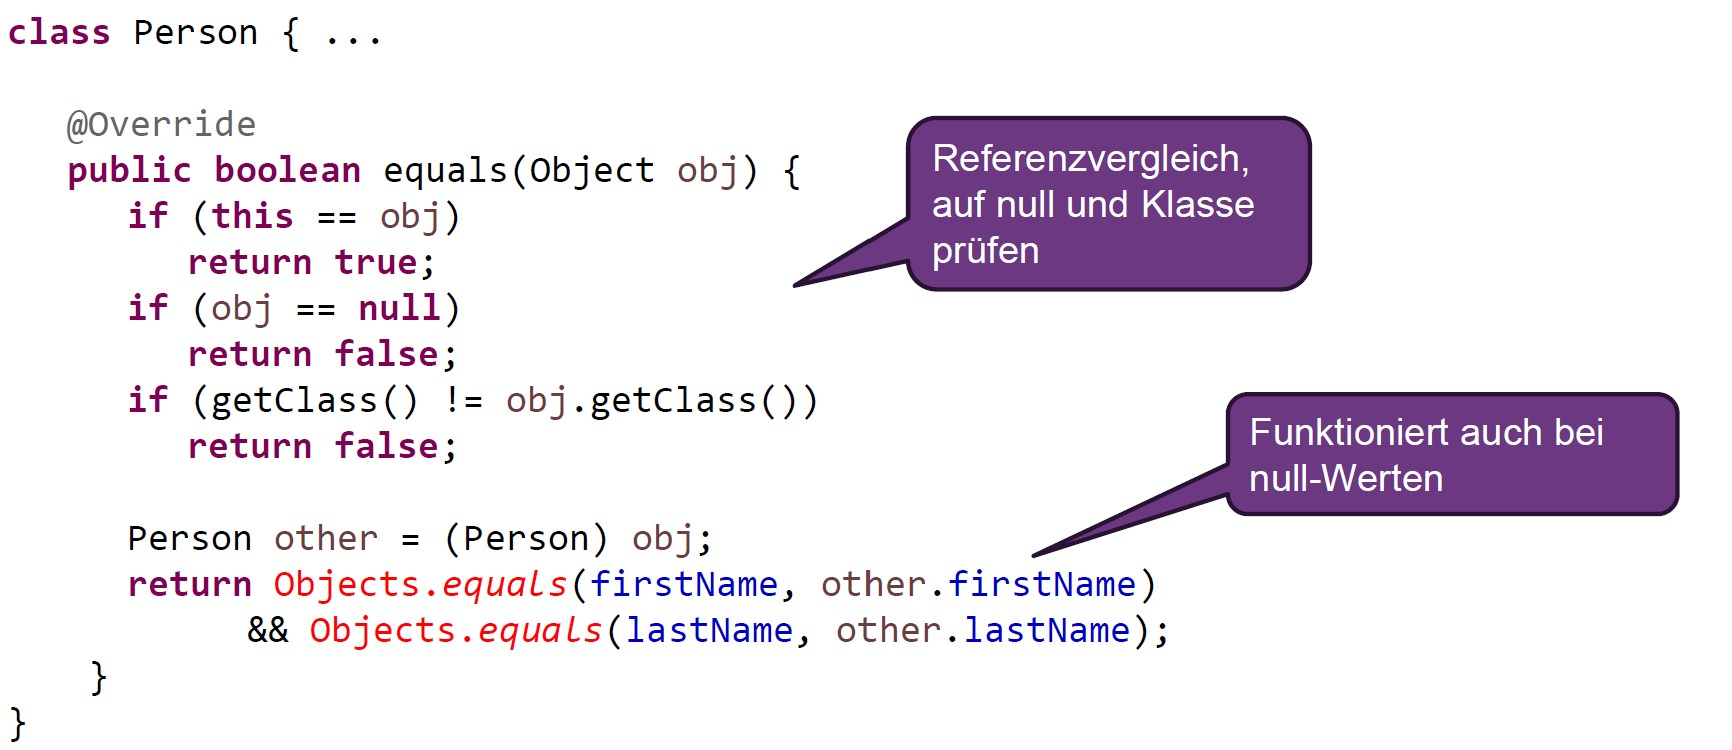
\includegraphics[width=\linewidth]{pictures/equals-impl.jpg}

\subsubsection{Hashing: Konzept}
Die Funktion \verb|hashCode()| bildet ein Objekt auf seinen Hash-Code ab, welcher den Ablegeort des Objekts definiert.\\
Gleiche Objekte können den gleichen Hashcode haben.\\
\textit{ACHTUNG : gleicher Hashcode muss aber nicht gleiches Objekt sein!}

\subsubsection{Hashfunktion}
Als Faustregel: Bei jedem \textbf{equals()} gleich ein \textbf{hashCode()} schreiben:\\
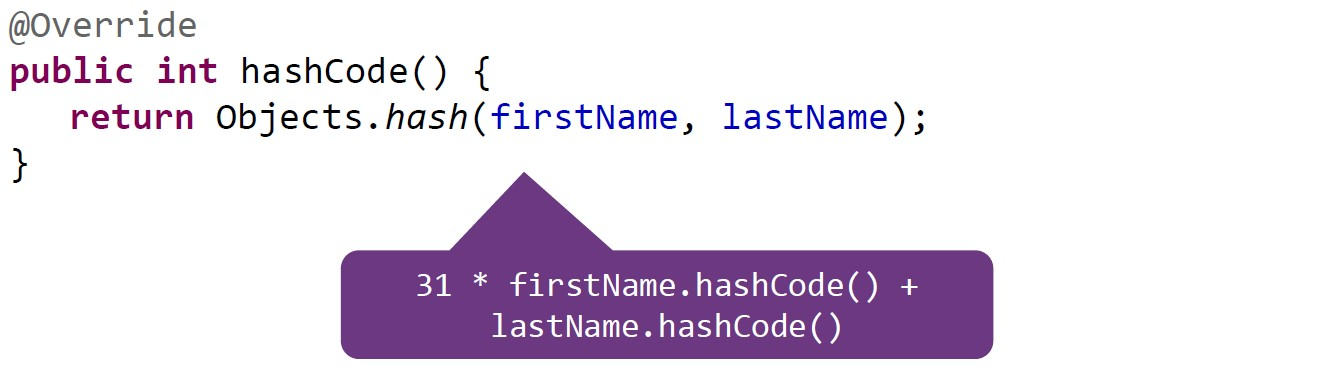
\includegraphics[width=\linewidth]{pictures/hashcode.jpg}